\section{Status}

Spring Boot is currently on version 2.20 as of October 16, 2019 with the following attributes on their GitHub repository at the time of writing \cite{github:online}:

\begin{itemize}
\item 23,886 commits
\item 137 releases
\item 628 contributors
\item 27,500 forks
\item Licensed under Apache 2.0
\end{itemize}

Based on a 2019 survey done by JetBrains on Java developers, Spring Boot was found to be very popular as shown by Figure ~\ref{fig:jb-survey-app-server} and ~\ref{fig:jb-survey-web-framework}.

\begin{figure}[H]
    \centering
    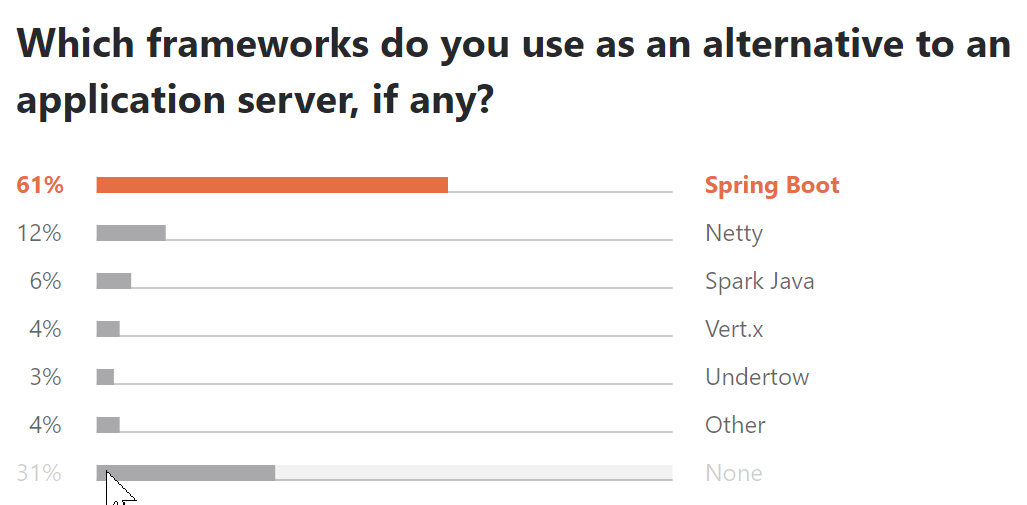
\includegraphics[width=0.75\textwidth]{content/introduction/jb-survey-app-server.png}
    \caption{JetBrains Survey Question About Java Application Server Usage \protect\cite{jetbrains:online}}
    \label{fig:jb-survey-app-server}
\end{figure}

\begin{figure}[H]
    \centering
    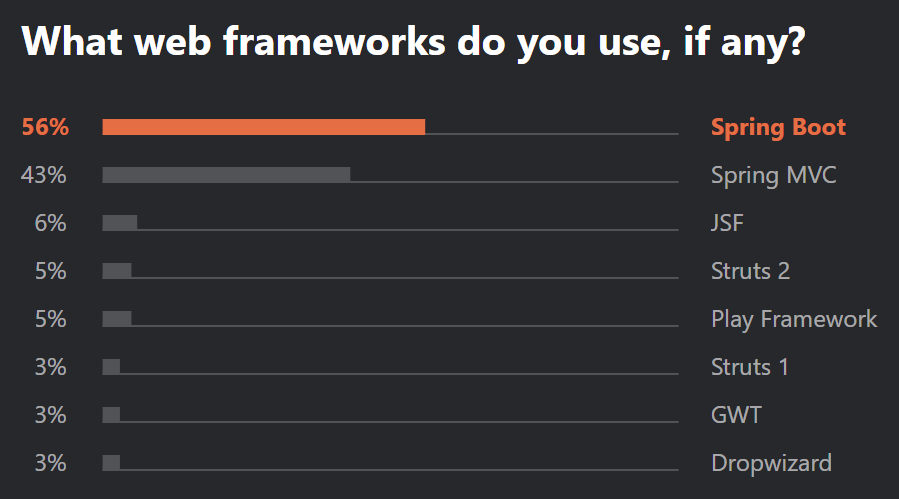
\includegraphics[width=0.75\textwidth]{content/introduction/jb-survey-web-framework.png}
    \caption{JetBrains Survey Question About Java Web Framework Usage \protect\cite{jetbrains:online}}
    \label{fig:jb-survey-web-framework}
\end{figure}

Both questions in the survey were overwhelmingly in favor of Spring Boot so can be easily written with confidence that Spring Boot is a familiar and heavily used Java framework. JetBrains adds that "Spring Boot has become the most popular Java web framework, adding 14\% since last year" \cite{jetbrains:online}.

